\documentclass[10pt]{scrreprt}
\usepackage[utf8]{inputenc}
\usepackage{amsfonts}
\usepackage{amsmath}
\usepackage{amssymb}
\usepackage{commath}
\usepackage[ngerman]{babel}
\usepackage{enumitem}
\usepackage{booktabs}
\usepackage{longtable}
\usepackage{relsize}
\usepackage{pgfplots}
\usepackage{csvsimple}
\usepackage{pgfplotstable}
\usepackage{siunitx}
\usepackage{fancyhdr}
\usepackage{color}
\usepackage{float}
\usepackage{listings}
\usepackage{graphicx}
\usepackage{subcaption}
\usepackage[europeanresistors]{circuitikz}

\definecolor{mygreen}{RGB}{28,172,0} % color values Red, Green, Blue
\definecolor{mylilas}{RGB}{170,55,241}


\lstset{language=Matlab,%
%basicstyle=\color{red},
breaklines=true,%
morekeywords={matlab2tikz},
keywordstyle=\color{blue},%
morekeywords=[2]{1}, keywordstyle=[2]{\color{black}},
identifierstyle=\color{black},%
stringstyle=\color{mylilas},
commentstyle=\color{mygreen},%
showstringspaces=false,%without this there will be a symbol in the places where there is a space
%numbers=left,%
%numberstyle={\tiny \color{black}},% size of the numbers
%numbersep=9pt, % this defines how far the numbers are from the text
emph=[1]{for,end,break},emphstyle=[1]\color{red}, %some words to emphasise
%emph=[2]{word1,word2}, emphstyle=[2]{style},
}

\setlength\parindent{0pt}

\setcounter{chapter}{4}
\setcounter{secnumdepth}{3}
\setcounter{section}{1}

\pagestyle{fancy}
\fancyhf{}
\lhead{GPET Versuch 9}
\rhead{Tim Luchterhand, Paul Nykiel}
\cfoot{\thepage}

\author{Tim Luchterhand, Paul Nykiel \protect\\ tim.luchterhand@uni-ulm.de, paul.nykiel@uni-ulm.de}
\title{GPET Versuch 9 --- Julius Edgar Lilienfeld}
\subtitle{Gruppe: Dienstag14}

\begin{document}
    \maketitle
    \section{Messung der Kennlinienfelder}
    In diesem ersten Versuchsteil sollen verschiedene Kennlinien für zwei unterschiedliche
    Transistoren aufgenommen werden.
    \begin{figure}[H]
        
\includegraphics[width=\textwidth]{abb12.png}
        \caption{Messaufbau zur Charakterisierung der FETs.}
        \label{fig:abb12}
    \end{figure}
    Hierzu verwenden Sie die Messschaltung nach Abb.~\ref{fig:abb12} T1 bezeichnet den Transistor
    BS270 und T2 den IPP60R950C6 von Infineon.
    \vspace{0.5cm}
    Nehmen Sie die Kennlinie $I_D = f (U_{GS} )\vert_{U_{DS}}$ auf. D.h. Sie messen den Drainstrom in
    Abhängigkeit von $U_{GS}$ bei konstanter Drain-Source-Spannung $U_{DS}$. Den Drainstrom $I_D$
    messen Sie mit einem Multimeter und achten Sie darauf einen Strom von $I_{D,\max} = 400\si{m\ampere}$
    nicht zu überschreiten. $U_{DS}$ halten Sie dabei konstant auf $3\si{\volt}$ (T1).
    Nehmen Sie für beide Transistoren 10 geeignete Messwerte auf und stellen Sie diese in
    einem Diagramm dar. (Bei T2 legen Sie für $U_{DS}$ konstant $4\si{\volt}$ an).

    \begin{enumerate}
        \item Wie groß ist jeweils $U_{TH}$?
        \item Bestimmen Sie Steilheit des Transistors T1 bei $40\si{m\ampere} \ldots 80\si{m\ampere}$.
    \end{enumerate}

    Im Weiteren nehmen Sie die Ausgangskennlinie $I_D = f (U_{DS} )\vert_{U_{GS}}$ der beiden Transistoren
    auf. Diesmal halten Sie $U_{GS}$ auf konstant $3\si{\volt}$ (T1) und erhöhen $U_{DS}$ schrittweise von $0$ bis
    $8\si{\volt}$. Überschreiten Sie $8\si{\volt}$ jedoch nicht und erzeugen Sie keine negativen $U_{DS}$. Nehmen
    Sie auch hier für beide Transistoren 10 geeignete Messwerte auf und stellen Sie diese in
    einem Diagramm dar. (Bei T2 müssen für $U_{GS} 4\si{\volt}$ anliegen). Sollten Sie einen Abriss
    der Kennlinie beobachten, ist dies entweder auf Überhitzung oder falsche Beschaltung
    zurückzuführen.

    Bestimmen Sie den Ausgangswiderstand $r_{DS}$ von T1 (Hinweis: Sättigungsbereich).

    \paragraph{Protokoll}
    $ $
    %TODO Zeugs, Formel bei 2.3, U_th, Steilheit,

    \begin{figure}[H]
        \centering
        \begin{tikzpicture}
    		\begin{axis}[ymin=0, xmin=0, xlabel = {$U_{GS}$[V]}, ylabel = {$I_D$[A]}]
    			\addplot[color=red] table[x index = {0},
                        y index = {1}] {42.csv};
                \addplot[color=blue] table[x index = {0},
                        y index = {1}] {42_2.csv};

    		\end{axis}
    	\end{tikzpicture}
        \caption{Eingangskennlinie. T1 in \textcolor{red}{Rot}, T2 in\textcolor{blue}{blau}.}
    \end{figure}

    Die Threshold-Spannung $U_{TH}$ ist die Spannung, ab dem ein Strom zu fließen
    beginnt und lässt sich aus der Eingangskennlinie bestimmen:

    \begin{eqnarray*}
        U_{T1,TH} &=& 1.74 \si{\volt}\\
        U_{T2,TH} &=& 3.51 \si{\volt}
    \end{eqnarray*}

    Bestimmung der Steilheit aus der Eingangskennlinie: Die Steilheit $G_m$
    entspricht der Steigung der Kennlinie unmittelbar nach $U_{TH}$. Zur Berechnungn wurden Werte zwischen
    $40\si{m\ampere}$ und $80\si{m\ampere}$ verwendet.

    \begin{equation*}
        G_m = \frac{0.07\si{\ampere} - 0.04\si{\ampere}}{2.552\si{\volt} - 2.360\si{\volt}} = 0.156\si{\siemens}
    \end{equation*}

    \begin{figure}[H]
        \centering
        \begin{tikzpicture}
    		\begin{axis}[ymin=0, xmin=0, xlabel = {$U_{DS}$[V]}, ylabel = {$I_D$[A]}]
    			\addplot[color=red] table[x index = {0},
                        y index = {1}] {42_3.csv};
                \addplot[color=blue] table[x index = {0},
                        y index = {1}] {42_4.csv};
    		\end{axis}
    	\end{tikzpicture}
        \caption{Ausgangskennlinie. T1 in \textcolor{red}{Rot}, T2 in\textcolor{blue}{blau}.}
    \end{figure}

    Der Ausgangswiderstand $R_{DS}$ lässt sich wie folgt bestimmen:

    \begin{equation*}
        R_{DS} = \frac{1}{Y_{out}}
    \end{equation*}

    Wobei sich $Y_{out}$ aus der Steigung der Kurve in der Ausgangskennlinie im
    Sättiungsbereich bestimmen lässt:

    \begin{eqnarray*}
        Y_{out} &=& \frac{0.125\si{\ampere} - 0.113\si{\ampere}}{4\si{\volt} - 2.024\si{\volt}} = 0.0061\si{\siemens}\\
        \Rightarrow R_{DS} &=& 164,67 \si{\ohm}
    \end{eqnarray*}

    \section{Verstärker} \label{sec:auf43}
    \begin{figure}[H]
        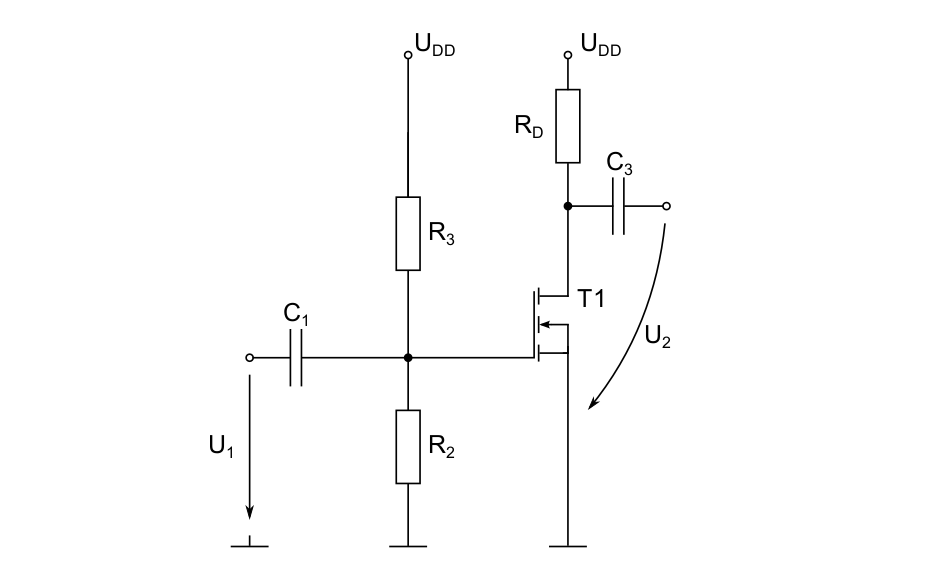
\includegraphics[width=\textwidth]{abb10.png}
        \caption{Verstärkernetzwerk}
        \label{fig:abb10}
    \end{figure}
    Bauen Sie nun die Verstärkerschaltung nach Abb.~\ref{fig:abb10} mit dem Transistor T1 (BS270) auf.
    Der Arbeitspunkt soll eine minimale Verlustleistung, einen großen Aussteuerbereich und
    einen hohen Ausgangswiderstand aufweisen. Der Betriebsmodus ist durch die Schaltung
    vorgegeben. Bauen Sie die Schaltung mit den folgenden Bauteilen auf: $C_1 = C_3 = 2.2\si{\mu \farad},
    R_D = 440\si{\ohm}, R_2 = 1.3\si{k\ohm}, R_3 = 10\si{k\ohm}$. Setzen Sie $U_{DD}$ auf $24\si{\volt}$. Bei korrekter
    Verschaltung sollte sich ein Drainstrom von ca. $50\si{m \ampere}$ ergeben. Schließen Sie den externen
    Funktionsgenerator, das Oszilloskop und die Spannungsversorgung an, nachdem Sie alle
    drei Geräte korrekt konfiguriert haben. Achten Sie besonders auf die Strombegrenzung
    der Spannungsversorgung.
    \begin{enumerate}
        \item Messen Sie den Amplitudengang $20 \text{dB} \cdot \log_{10} \left( \dfrac{U_2(f)}{U_1(f)} \right)$
            \begin{enumerate}
                \item für Frequenzen zwischen $100\si{\hertz}$ und $4\si{M\hertz}$.
                \item mit 2 Messpunkten pro Dekade.
                \item Frequenzgenerator: $100 \si{m\volt}_{pp}$, Sinus, deaktivierter Offset.
                \item Achten Sie bei höheren Frequenzen auf einen möglichen Abfall dieser
                    Eingangsamplitude. Regeln Sie bei Bedarf nach.
            \end{enumerate}
        \item Stellen Sie den gemessenen Amplitudengang in einem Diagramm dar. Wie groß ist
            $A_V$ bei $1\si{k\hertz}$?
    \end{enumerate}
    Die Bandbreite eines Verstärkers ist definiert als 3 dB Abfall der Verstärkung im Vergleich
    zu niedrigen Frequenzen, die als DC angenommen werden können, bzw.\ als Reduzierung
    der Ausgangsspannung $U_2$ um den Faktor $\frac{1}{\sqrt{2}}$. Ein Betrieb des Verstärkers jenseits seiner
    Bandbreite ist gewöhnlich nicht zu empfehlen, da er seine Funktion in diesem
    Frequenzbereich nicht mehr erfüllen kann.
    \begin{enumerate}
        \setcounter{enumi}{2}
        \item Wie groß ist die Bandbreite des Verstärkers?
    \end{enumerate}

    \paragraph{Protokoll}
    $ $
    \begin{figure}[H]
        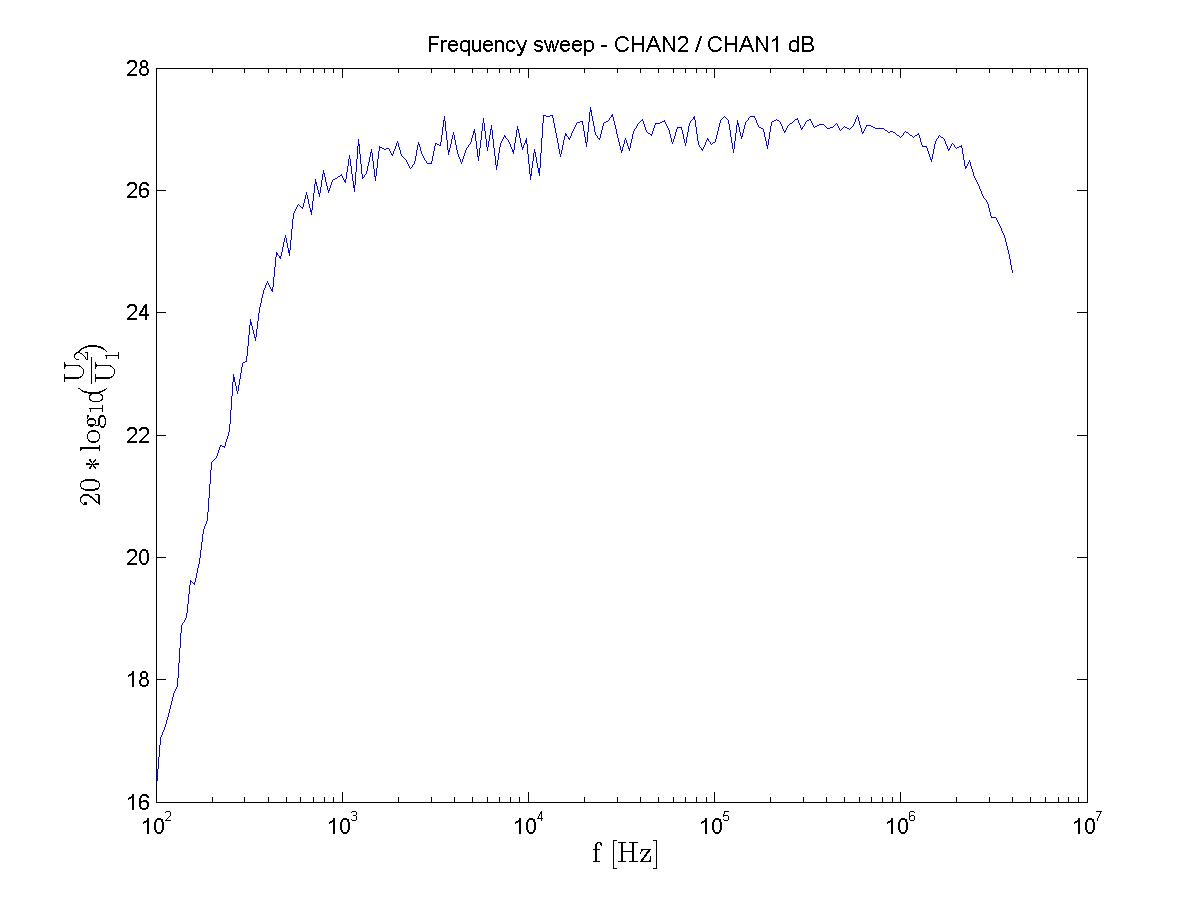
\includegraphics[width=\textwidth]{BS43_frequencysweep_ylogxlog.jpg}
        \caption{Frequenzgang des Verstärkers}
        \label{}
    \end{figure}

    Durch Ablesen erhält man:
    \begin{equation*}
        A_v(1\si{k\hertz}) = 26.1 \text{dB}
    \end{equation*}

    Die Bandbreite lässt sich folgndermaßen bestimmen: Die maximale Verstärkung
    beträgt ca.~27dB. Also ist die Bandbreite der Bereich, in dem die Verstärkung
    überhalb der 24dB Marke liegt. Dieser Bereich geht von ca.~$1.25 \cdot 10^2 \si{\hertz}$
    bis $1.3 \cdot 10^6 \si{\hertz}$.

    \section{Class-A Endstufe}
    \begin{figure}[H]
        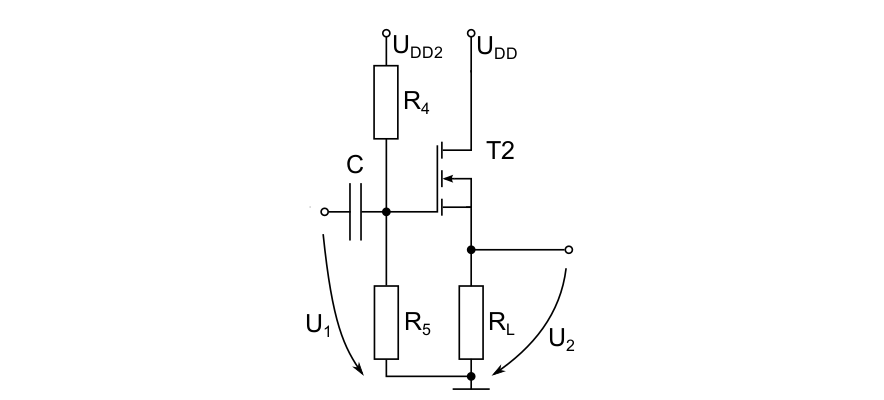
\includegraphics[width=\textwidth]{abb11.png}
        \caption{Class-A Endstufe}
        \label{fig:abb11}
    \end{figure}
    Bauen Sie nun die Endstufe nach Abb.~\ref{fig:abb11} mit dem Transistor T2 (IPP 60) auf. Der
    Widerstand $R_L$ der Kopfhörer beträgt $40\si{\ohm}$ pro Kanal. Wählen Sie einen entsprechenden
    Widerstand von $47\si{\ohm}$ für ihre Messungen. Erst im letzten Schritt wird der Sourcewiderstand
    durch den Kopfhörer ersetzt. Diese einfache Endstufe weist eine hohe Verlustleistung auf,
    die in der angeschlossenen Last in Wärme umgewandelt wird. Um die Kopfhörer nicht zu
    beschädigen, soll $I_D$ auf $100\si{m\ampere}$ begrenzt werden.
    \begin{enumerate}
        \item Bauen Sie die Schaltung auf mit $U_{DD} = 7\si{\volt}, U_{DD2} = 7\si{\volt}, Z_L = 47\si{\ohm}, R_5 = 1\si{M\ohm}$ und
            $R_4 = 100\si{k\ohm}, C = 2.2\si{\mu \farad}$, regeln Sie bei Bedarf $U_{DD2}$ nach, um $I_D auf 100\si{m\ampere}$ zu
            beschränken.
        \item Messen Sie die Verstärkung bei $20\si{k\hertz}$ und einer Ausgangsamplitude des
            Frequenzgenerators von $500\si{m\volt}\ (1\si{\volt}_{pp})$, Sinus.
        \item Bauen Sie nun einen vollständigen Signalpfad bestehend aus Verstärker und
            Endstufe, indem Sie den Ausgang des Verstärkers aus Teilaufgabe~\ref{sec:auf43} mit dem Eingang
            der Endstufe über den Koppelkondensator $C$ verbinden.
        \item Ersetzen Sie den Sourcewiderstand durch den Kopfhörer (regeln Sie unter
            Umständen $U_{DD2}$ nach, um $I_D$ auf $100\si{m\ampere}$ zu beschränken - achten Sie beim Verwenden der
            Kopfhörer auf die Lautstärke --- setzen Sie die Kopfhörer erst auf, wenn die
            Schaltung funktioniert!) und fahren Sie langsam das Frequenzintervall $50\si{\hertz} \ldots 20\si{k\hertz}$
            durch bei einer Lastamplitude von $500\si{m\volt}$, Sinus. Sie sollten einen entsprechenden
            störfreien Ton hören. $440\si{\hertz}$ entsprechen dem Kammerton ’a’ (eingestrichenes a),
            der als Referenz zum Einstimmen von Musikinstrumenten verwendet wird.
    \end{enumerate}

    \paragraph{Protokoll}
    \begin{figure}[H]
        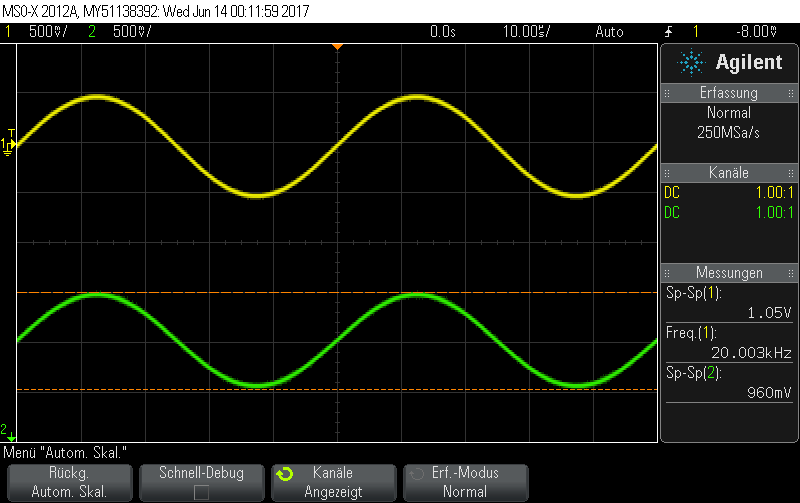
\includegraphics[width=\textwidth]{scope_1.png}
        \caption{Verstärkung bei $20\si{k\hertz}$}
        \label{fig:Enstufe}
    \end{figure}

    Die Endstufe dient lediglich als Stromverstärker, um einen kleinen Lastwiderstand
    betreiben zu können, ohne die Funktionalität des Vorverstärkers zu beeinträchtigen.
    Die Endstufe verstärkt also nicht die Spannung. Dies ist auch in Abbildung
    \ref{fig:Enstufe} zu erkennen, da hier die Amplituden der Ein- und Ausgangssignale
    quasi gleich groß sind.

\end{document}
